\section{Simulation Model and Implementation} \label{sec:methods}

% Experiments were conducted \textit{in silico} using stochastic agent-based modeling approaches.
Our simulations tracked fixed-capacity populations of discrete agents propagated in synchronous generations, with competition between agents to create asexual offspring.
Each agent possessed a set of genetic traits, inherited subject to mutation, that influenced reproductive success; mutator strains were subjected to 100$\times$ higher mutation rates.
Our genome model tracked counts of accumulated beneficial and deleterious mutations, following closely from \citep{raynes2018sign}.
To assess the generality of our findings, we supplemented this simple ``counter-based'' genome model with an alternate ``site-explicit'' genome model where beneficial mutations become rarer as adaptation unfolds.
% These genome models are described below.
%
% This section reviews the model mechanics used across experiments in this work, as well as aspects of simulation design used to enact treatment conditions.
% Experimental variables varied between treatments include population size, spatial population structure, background prevalence of mutator traits, and restriction of adaptive potential.
% Finally, we describe notable implementation-level considerations necessary in harnessing high-performance computing hardware to achieve the simulation of large, heterogeneous populations necessary for this work.
%
% \subsection{Counter-based Genome Model} \label{sec:poisson}
%
% Primary experiments in this work apply an agent-based modeling approach closely following work by \citet{raynes2018sign}.
% We also adopt parameters from \citet{raynes2018sign}, which were chosen on the basis of values reported from laboratory measurements on \textit{E. coli} strains\citep{wloch2001direct,frenkel2014fates,joseph2004spontaneous,levy2015quantitative,zeyl2001estimates}.
% Under the ``counter-based'' framework, agent genomes consist of two counters: one tracking beneficial mutations accumulated ($n_b$) and the other tracking deleterious mutations accumulated $n_d$.
% As modeled in several pieces of related work \citep{tenaillon1999mutators,travis2002mutator,raynes2019migration,tanaka2003evolution,wylie2009fixation}, mutations are assumed to have comparable fitness impacts.
% Thus, a genome's ``fitness score'' is calculated simply as $n_b - n_d$.
% (Details on how ``fitness score'' influences selection are described in Section \ref{sec:evolution}.)
% For purposes here, the simplicity of this approach is useful in enabling runtime simulation efficiency.
% Sensitivity analysis performed in closely related work applying this genome model found evolutionary outcomes to be similar to those with exponential distributions of fitness effects for individual mutations \citep{raynes2019selection}.
%
% Genomes were subjected to mutation each generation.
% For each offspring, counts of newly accrued beneficial and deleterious mutations are drawn from independent Poisson distributions.
% Expected deleterious mutations per generation were parameterized as
% $\lambda_d=10^{-3}$ and expected beneficial mutations per generation were parameterized as $\lambda_b=10^{-6}$.
% Reversions are not considered, so beneficial and deleterious mutation counts are strictly nondecreasing.
% In some experiments where adaptive potential was limited, we imposed an upper bound on the maximum quantity of beneficial mutations available.
% Any further beneficial mutations accrued past this point were reverted to the bound.
%
% Agent genomes additionally contain a boolean flag, signifying whether the agent expresses a mutator trait.
% Agents with this trait incur a hundred-fold increase to mutation rates, $\hat{\lambda_d} = 100 \times \lambda_d$ and $\hat{\lambda_b} = 100 \times \lambda_b$.
% We assume no direct fitness benefit or cost to be associated with the mutator allele.
%
% Experiments applied one of two approaches to introduce mutator alleles.
% In the ``50/50'' treatment, genomes were initialized equiprobably as a mutator or as a nonmutator.
% The ``50/50'' experiment design, applied in \textit{in vivo} experiments reported in \citet{raynes2018sign}, maximizes sensitivity in detecting sign-change fitness effects where selection transitions between favoring versus disfavoring mutator alleles.
% Rationale behind this approach also stems from the understanding that fitness effects from mutator alleles act in a density- and count-independent manner \citep{raynes2019selection}.
% By contrast, in other experiments, we introduced mutator alleles via a \textit{de novo} approach where the mutator trait is spontaneously conferred to offspring with probability $10^{-6}$.
% Under this approach, the founding population is initialized as nonmutator type.
% As with prior work \citep{raynes2018sign}, neither treatment allows mutator to nonmutator reversion.
%
% \subsection{Site-explicit Genome Model} \label{sec:site-explicit}
% As originally formulated in \citet{raynes2018sign}, the counter-based genome model assumes the availability of an unlimited adaptive potential.
% In particular, the memorylessness of the probability distribution for mutation accumulation suits the assumption that an unlimited number of beneficial (or deleterious) mutations are available.
% To better reflect scenarios with limited adaptive potential, we replicated several experiments using a genome model explicitly designating a finite set of loci with adaptive potential.
% The major consequence of such a ``site-explicit'' model is that discoverable beneficial mutations become scarcer, and hence more difficult to discover, as adaptation unfolds.

% Under the site-explicit approach, we model genomes as containing a discrete, finite set of $n$ loci $b_i \in \{0, 1\}$ available for adaptive mutation.
% All loci are initialized $b_i = 0$.
% When inherited, loci transition $0 \rightarrow 1$ with probability $p_b = 10^{-6}$, representing acquisition of a beneficial mutation.
% Reversion mutations $1 \rightarrow 0$ are allowed, also with probability $p_{\sim b} = 10^{-6}$.

% Because we do not limit the quantity of available deleterious mutations in our simulations, we maintained a counter-based approach in tracking deleterious mutations, with deleterious mutation acquisition Poisson distributed $\lambda_d = 10^{-3}$.
% Hence, under the site-explicit model, we assign agents' fitness scores as $-n_d + \sum^n b_i$.

% Mutator allele mechanics under the site-explicit model closely follow the counter-based model.
% The mutator trait increases mutation rates hundredfold, setting $\hat{p_{b}} = \hat{p_{\sim b}} = 10^{-4}$ and $\hat{\lambda_d} = 10^{-1}$.
% Site-explicit experiments were conducted under both ``50/50'' and ``\textit{de novo}'' models of mutator introduction, identically to description above.

% \subsection{Evolution Model} \label{sec:evolution}

% Simulations applied a tournament selection strategy with synchronous generations and fixed population size.
% For each available slot in a subpopulation's next generation, we sampled, with replacement, a pair of candidate parents from that subpopulation.
% With 90\% probability, a selected parent is chosen randomly among the pair.
% Otherwise, the candidate with the higher fitness score was selected as the parent.
% As such, fitness score improvements conferred a 10\% fitness advantage.
% Our motivation in performing selection via pairwise competition was to enable efficient vectorized operations for GPU evaluation.

% In simulations with spatial structure, populations were partitioned into well-mixed 256-agent ``demes.''%
% \footnote{%
% Where noted, 32-agent and 2,048-agent deme sizes were also used, to support finer-grained sweeps of population size or higher maximum net population size.
% }
% Where deme structure was used, competition occurred only between agents inhabiting the same deme.
% Each generation, migration between neighboring demes was applied by swapping a pair of agents.
% Hence, demes received one immigrant from each neighbor per generation.
% Under default conditions, demes were arranged as a two-dimensional grid lattice with non-toroidal boundaries (i.e., grid edges did not wrap around).
% For well-mixed treatments, deme structure was broken down to treat entire populations as a single deme.

% Our 2D structure experiments used square deme grids.
% To maintain square layout, we scaled surveyed population sizes by factors of 9: $1 \times 1 \times 256,\;\; 3 \times 3 \times 256,\;\; 9 \times 9 \times 256,\;\; \ldots,\;\; 729 \times 729 \times 256$.
% To efficiently batch our computations, we processed smaller population sizes as independent tiles of a larger, fixed-size fabric.
% Hence, replicate count decreased with population size, but was boosted to at least 9 replicates in all cases.
% Simulations lasted 500,000 generations, which sufficed for populations to reach fixation in nearly all cases.
% (We defined fixation as all mutators or all nonmutators for 50/50 experiments, and as either 100\% mutators or <1\% mutators for \textit{de novo} experiments.)
% However, we found that 256-agent populations failed to reliably reach full adaptive potential in accruing more than 12 beneficial mutations within the prescribed 500,000 generation window.
% Thus, we excluded 256-agent simulations with more than 12 beneficial mutations available from our analyses.

% For all included data, $>97\%$ of replicates reached both mutator/nonmutator fixation and accrued full adaptive potential.
% Details on the fraction of replicates reaching fixation by experimental condition are provided in Supplementary \cref{fig:neither-fixed-5050-cupy,fig:neither-fixed-denovo-cupy,fig:neither-fixed-wse-256atile,fig:neither-fixed-wse-altatile}.
% Details on the fraction of replicates reaching full adaptive potential, measured for GPU-based simulations, appear in Supplementary \cref{fig:unaccrued-5050-cupy,fig:unaccrued-denovo-cupy}.

% \subsection{Hardware Accelerator Platforms} \label{sec:hardware}

% \subsection{Kernel Design} \label{sec:kernel}

To suit the local lattice structure of the WSE's hardware architecture, all experiments on this platform employed 2D spatial population structure.
Each PE hosted a single subpopulation, acting as an ``island.''
Thus, in trials configured with 2,048 agents per PE, net population size reached 1.5 billion agents.
Agents migrated between neighboring PEs via asynchronous message passing;
% see e.g.,
% https://github.com/mmore500/wse-async-ga/blob/ebc92bd012f0bb31092c5e71825af041261c35c5/kernel-async-ga/kernel.csl
% and
% https://osf.io/esv9z
% (note that send flag is bumped twice per send cycle)https://osf.io/esv9z
in practice, each PE dispatched approximately one agent to each neighbor per generation.
Progress of each PE in stepping through agent generations within its own subpopulation was allowed to proceed independently of other PEs.
Other detail on the Cerebras Software Language (CSL) kernel design adapted for this work is provided in \citet{moreno2024trackable}.

% In some cases, experiments on WSE were extended beyond the $729 \times 729$ deme configuration to fill the CS-2 WSE's entire $750 \times 994$ complement of available PEs.

% For a set of supplementary trials described in Section \ref{sec:dynamics}, we applied additional runtime data logging in our simulations to track time series data of mutator allele prevalence.
% Generation-on-generation, we configured each processor element to sample a genome from its local population and record its mutator allele status (i.e., a binary value as either a non- or mutator).
% To efficiently curate this single-bit data within per-PE memory limits while allowing a flexible recording duration, we leveraged recently introduced ``DStream'' ring buffer data structures \citep{moreno2024algorithms}.
% Notably, this approach constrained memory use to a fixed-size buffer, while allowing recording to be dynamically halted when nonmutators were determined to be locally extinct (and restarted if they are reintroduced).
% While this scheme allowed maximization of on-device resources, as a consequence the set of sampled time points varied depending on how long nonmutator alleles persisted.
% As a result, the number of generations elapsed per frame in provided animations varies. Availability


% Given the stochastic nature of agent-based evolution models, our experiments relied heavily on pseudorandom number generators (PRNGs).
% These algorithms emulate true entropy by producing a sequence of output values that, although deterministic, are statistically independent.
% Due to performance engineering considerations, vendor-supplied PRNG implementations for the WSE and GPU do not employ cryptographic-quality algorithms.
% Our WSE simulations relied on Cerebras Software Language's PRNG utilities, which use a Linear-Feedback Shift Register (LFSR) approach with polynomial $3x^2 + 8x + 1$ strided by 128 iterations.
% On GPU, we used CuPy's PRNG utilities, which expose CUDA's underlying XORWOW-based CuRAND implementation \citep{marsaglia2003xorshift}, another type of LFSR approach \citep{brent2004note}.

% PRNG patterning, particularly in lower-quality Linear Congruential Generator (LCG) algorithms, has been shown in some cases to substantially bias simulation results \citep{click2010quality}.
% Notably, we encountered one set of conditions in WSE simulations where fixation probabilities for 12 beneficial mutations available deviated appreciably from that for 10 and 14 beneficial mutations.
% The anomaly occurred solely under the site-explicit genome model, where the number of PRNG calls made to apply mutation to an agent differs with the quantity of available beneficial mutations.
% In the anomalous configuration, each PE comprised a fully independent population, so replicate count was very high ($n = 827 \times 827 = 683,929$), making the result all the more unexpected.

% Fully re-running the affected simulation did not resolve the data anomaly.
% However, modifying the simulation code to advance the PRNG engine via no-op calls within the body of the mutation operator brought the result in line with expectations.
% Thus, it seems likely that, in this instance, the simulation encountered a PRNG cycle or similar artifact.
% As such, for this data point, we exclude the originally generated data in favor of the results with added PRNG stepping.
% We note that on a more general basis, the soundness of our simulation implementations is bolstered by consistency between similar experiments conducted on WSE and GPU.
% In particular, CuRAND's RNG has been extensively characterized and, although it exhibits statistically detectable flaws of its own, is considered to be of production quality \citep{nvidia2024curand}.
% Given the stochastic nature of agent-based evolution models, our experiments relied heavily on pseudorandom number generators (PRNGs).
% These algorithms emulate true entropy by producing a sequence of output values that, although deterministic, are statistically independent.
% Due to performance engineering considerations, vendor-supplied PRNG implementations for the WSE and GPU do not employ cryptographic-quality algorithms.
% Our WSE simulations relied on Cerebras Software Language's PRNG utilities, which use a Linear-Feedback Shift Register (LFSR) approach with polynomial $3x^2 + 8x + 1$ strided by 128 iterations.
% On GPU, we used CuPy's PRNG utilities, which expose CUDA's underlying XORWOW-based CuRAND implementation \citep{marsaglia2003xorshift}, another type of LFSR approach \citep{brent2004note}.

% PRNG patterning, particularly in lower-quality Linear Congruential Generator (LCG) algorithms, has been shown in some cases to substantially bias simulation results \citep{click2010quality}.
% Notably, we encountered one set of conditions in WSE simulations where fixation probabilities for 12 beneficial mutations available deviated appreciably from that for 10 and 14 beneficial mutations.
% The anomaly occurred solely under the site-explicit genome model, where the number of PRNG calls made to apply mutation to an agent differs with the quantity of available beneficial mutations.
% In the anomalous configuration, each PE comprised a fully independent population, so replicate count was very high ($n = 827 \times 827 = 683,929$), making the result all the more unexpected.

% Fully re-running the affected simulation did not resolve the data anomaly.
% However, modifying the simulation code to advance the PRNG engine via no-op calls within the body of the mutation operator brought the result in line with expectations.
% Thus, it seems likely that, in this instance, the simulation encountered a PRNG cycle or similar artifact.
% As such, for this data point, we exclude the originally generated data in favor of the results with added PRNG stepping.
% We note that on a more general basis, the soundness of our simulation implementations is bolstered by consistency between similar experiments conducted on WSE and GPU.
% In particular, CuRAND's RNG has been extensively characterized and, although it exhibits statistically detectable flaws of its own, is considered to be of production quality \citep{nvidia2024curand}.
% \subsection{On-hardware Simulation Performance}
% \label{sec:performance}

% \begin{figure}

% \begin{subfigure}{0.5\textwidth}
% 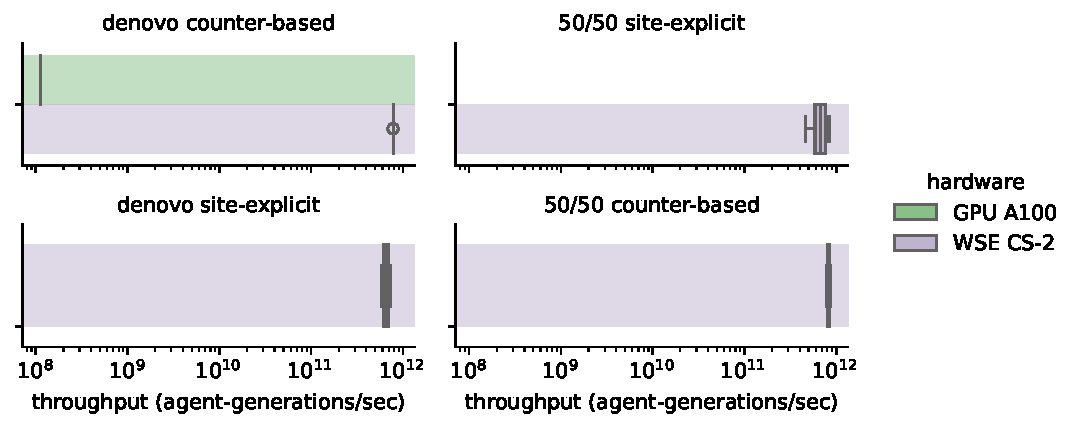
\includegraphics[width=\textwidth, trim={0cm 0cm 2.5cm 0cm}, clip]{binder/binder-perf-wse-vs-gpu.ipynb/binder/teeplots/col=experiment-design+hue=hardware+orient=h+viz=backplot+x=throughput-agent-generations-sec+ext=.pdf}
% \caption{throughput}
% \label{fig:perf:throughput}
% \end{subfigure}%
% \begin{subfigure}{0.49\textwidth}
\centering
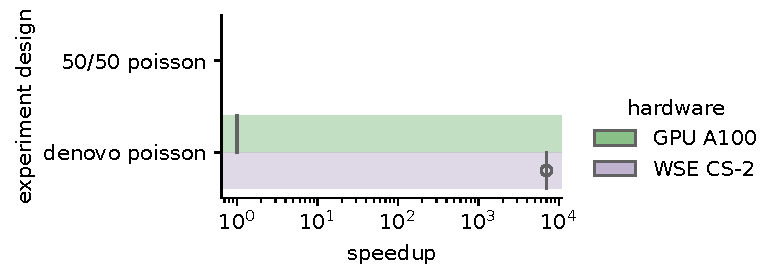
\includegraphics[width=0.85\linewidth]{binder/binder-perf-wse-vs-gpu.ipynb/binder/teeplots/hue=hardware+orient=h+viz=backplot+x=speedup+y=experiment-design+ext=.pdf}

\vspace{-2ex}
% ~
% \caption{speedup}
% \label{fig:perf:speedup}
% \end{subfigure}

\caption{
  \textbf{CPU, GPU, and WSE simulation performance.}
  \footnotesize
  CPU throughput was measured from NumPy-backed simulation code, GPU throughput was measured from equivalent CuPy-backed simulation code, and WSE throughput was measured from a comparable Cerebras Software Language implementation.
  CPU experiments were single-core on AMD EPYC 7H12 (2.595 GHz), GPU hardware was NVIDIA A100 hosted by AMD EPYC 7713 (2.0 GHz) or Intel Xeon 8358 (2.6 GHz), and WSE hardware was CS-2 hosted by Intel Xeon Platinum 8280L (2.7-4.0 GHz).
  Speedup was calculated relative to mean CPU throughput.
  % Shaded areas indicate bootstrapped 95\% confidence intervals with sample size $\geq 10$.
}
\label{fig:perf}
\end{figure}


% To assess the efficacy of hardware accelerator resources in expediting our simulations, we collected timings of runtime duration from our simulation experiments.
% As a baseline comparison point for performance, we also benchmarked simulation on CPU (AMD EPYC 7H12 2.595 GHz).

% Figure \ref{fig:perf} compares simulation performance between hardware platforms, measured in agent-generations per second (AGPS).
% Mean throughput was 7.0 (SD 0.5) million AGPS on CPU, 2.7 (SD 0.03) billion AGPS on GPU, and 780 (SD 0.5) billion AGPS on WSE for \textit{de novo} trials using the counter-based model.
% Net speedup, normalized to mean CPU throughput, was $378\times$ (SD 4) on GPU and $111,091\times$ (SD 75) on WSE.
% Normalized to net GPU performance, WSE provided a speedup of $294\times$ (SD 0.2).

% Under the site-explicit model, WSE gave 650 (SD 50) billion AGPS under \textit{de novo} conditions.
% The site-explicit model was not implemented on GPU.
% For all the above, 50/50 trials gave similar performance to \textit{de novo}.

% On WSE, we found agent-generation throughput to be generally consistent across per-PE population densities, as shown in Supplementary Figure \ref{fig:perf-tilepop}.
% In contrast, mean GPU throughput dropped $>95\%$ to 121 million AGPS when increasing net population size from 15.1 million to 175 million.
% For this reason, we only scaled GPU experiments up to 15.1-million-agent populations ($243 \times 243$ demes).

% \subsection{Software, Data, and Materials} \label{sec:materials}

Simulation code, configuration files, and batch scripts are available via the Open Science Framework at \url{https://doi.org/10.17605/OSF.IO/YMAF8}.
% To enable the simulation scale necessary for this work, we employed Graphics Processing Unit (GPU) and Wafer-Scale Engine (WSE) hardware accelerators, which contain large collections of worker processors specialized for numerical computation.
CPU hardware was AMD EPYC 7H12, GPU hardware was NVIDIA A100, WSE hardware was Cerebras CS-2 \citep{buitrago2021neocortex,Brashear2025}.
%\citep{choquette2021nvidia,cerebras2021wafer}.
% WSE hardware was hosted by the Neocortex at PSC.

% This project benefited significantly from open-source scientific software \citep{2020SciPy-NMeth,harris2020array,reback2020pandas,mckinney-proc-scipy-2010,waskom2021seaborn,hunter2007matplotlib,moreno2023teeplot}.
